\chapter{Панель Администратора}
\label{sec:chapter_admin}

В системе WordPress существует административная консоль системы управления сайтом, где вебмастер может добавлять или изменять контент своего блога, а также проводить различные изменения и усовершенствования по дизайну и функциям сайта.

Для входа в консоль администратора откройте страницу по адресу http://\MainDomain /wp-login.php (см. рис. \ref{fig:pic_Login})

\begin{figure}[htp]
    \centering
	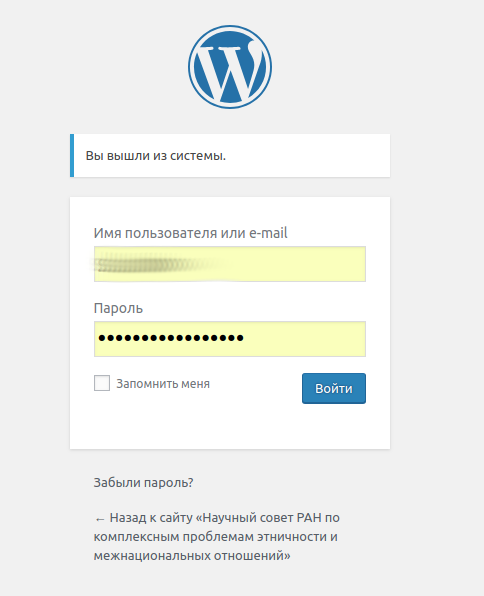
\includegraphics[width=0.3\textwidth]{login.png}
    \caption{Вход в Систему}
    \label{fig:pic_Login}
\end{figure}


После входа в систему откроется консоль администратора сайта (см. рис. \ref{fig:pic_welcome})

\begin{figure}[htp]
    \centering
	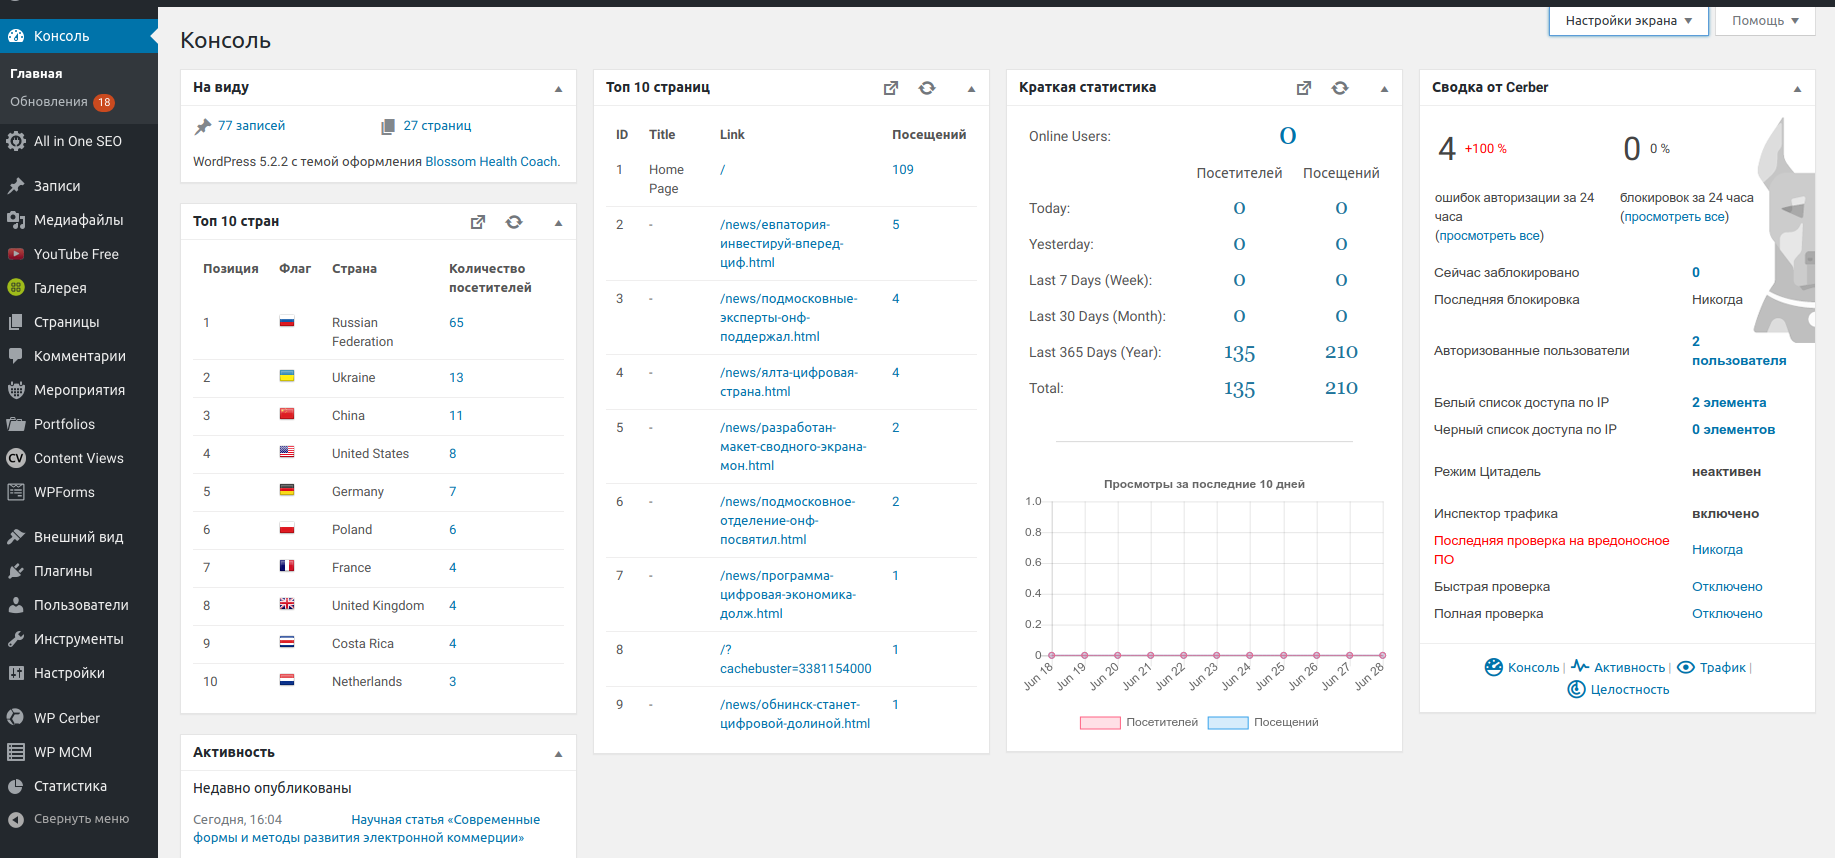
\includegraphics[width=\textwidth]{welcome.png}
    \caption{Стартовая страница администратора}
    \label{fig:pic_welcome}
\end{figure}

В правом верхнем углу есть кнопка «Настройки экрана». С ее помощью можно настроить все, что должно отображаться на странице.

Из перечисленного списка можно выбрать свежие комментарии, плагины, входящие ссылки, быструю публикацию, свежие черновики, блог, другие новости WordPress.

Слева на главной странице админки WordPress расположено вертикальное меню основных функций, которыми может воспользоваться вебмастер, его можно свернуть или развернуть.

К примеру, чтобы добавить запись, нужно перейти в раздел «Записи». В разделе «Внешний вид» устанавливается дизайн сайта, виджеты, меню, а также располагается редактор HTML. Не менее важны разделы «Плагины», «Инструменты» и «Параметры».

\section{Настройки}
\label{sec:part_wp_settings}

Настройки в админ панели WordPress, находятся в разделе «Параметры» — это самый важный раздел, в котором следует разобраться в первую очередь.

При нажатии на «Параметры» открывается выпадающее меню, которое содержит следующие группы настроек:

\begin{itemize}
\item Общие;
\item Написание;
\item Чтение;
\item Обсуждение;
\item Медиафайлы;
\item Постоянные ссылки.
\end{itemize}

\subsection{Общие настройки}
\label{sec:part_wp_settings_common}

В данном разделе вебмастер может задать название блога и его описание, которые будут находиться на основной странице сайта, а также использоваться в выдаче поисковых систем.
Следующий пункт в разделе «Общие» это адрес сайта и адрес WordPress. Рекомендуется указать одинаковый адрес, идентичный URL, чтобы в дальнейшем это не вызвало путаницы.

После этого в соответствующем поле вебмастер может указать свой действующий e-mail адрес, куда будут приходить все уведомления от WordPress, будь то свежие комментарии или обновленные настройки.

Затем следует очень интересный пункт под названием «Членство». Ставя под ним галочку, вебмастер разрешает регистрацию пользователей на своем ресурсе, но если смотреть объективно, данная функция бывает полезна владельцам блогов довольно редко.

В завершении общих настроек можно выбрать необходимый часовой пояс, формат даты и времени.

\subsection{Написание}
\label{sec:part_wp_settings_write}

В разделе «Написание» вебмастер может настроить отложенную публикацию и публикацию через e-mail адрес.
Здесь лучше оставить все как есть, потому, что большинству пользователей данная функция не пригодится.

\subsection{Чтение}
\label{sec:part_wp_settings_read}

В разделе «Чтение» владелец сайта может настроить страницу, которая будет главной. Это может быть статическая страница или последние записи на блоге. В роли статической главной страницы может выступать домашняя страница или любая другая, в том числе и специально созданная автором блога.
В данном разделе можно настроить, количество записей, которые будут отображаться на одной странице. А также настроить количество элементов, которые будут отображаться в RSS записях.

Последним пунктом в разделе является «Видимость для поисковых систем». Галочку здесь ставить не нужно, иначе сайт не будет проиндексирован.

\subsection{Обсуждение}
\label{sec:part_wp_settings_blog}

В разделе «Обсуждение» настраивается все, что так или иначе связано с комментариями. Это настройки по умолчанию, другие настройки комментариев, настройки отправления письма, модерация комментариев.
Медиафайлы

В разделе «Медиафайлы» владелец блога может задать необходимую ширину и высоту миниатюры изображений, а также максимальную ширину и высоту для изображений средних и крупных размеров.

\subsection{Постоянные ссылки}
\label{sec:part_wp_settings_links}

«Постоянные ссылки» — один из самых важных разделов админки wordpress. Здесь вебмастер имеет возможность настроить вид отображаемой ссылки, который больше всего для него подходит.

Ссылка может иметь название по умолчанию, может быть в виде даты и названия записи, месяца и названия записи, в виде цифр, названия или иметь произвольный формат.

Самым оптимальным вариантом является ссылка в виде одного названия. Так, владелец сайта может давать название ссылки идентичное названию статьи, только латинскими символами.

Это дает сайту огромное преимущество в поисковой выдаче, к тому же ссылки в виде названий статьи более приятны для посетителей сайта.

